\chapter{Energieversorgung}
\label{chap:Energieversorgung}
Für die Betrachtung von Smart Contracts in der Energieversorgung, eignet sich das lokal in Kempten ansässige Unternehmen Allgäuer Überlandwerk (AÜW).

\begin{wrapfigure}{r}{0.5\textwidth}
\centering
  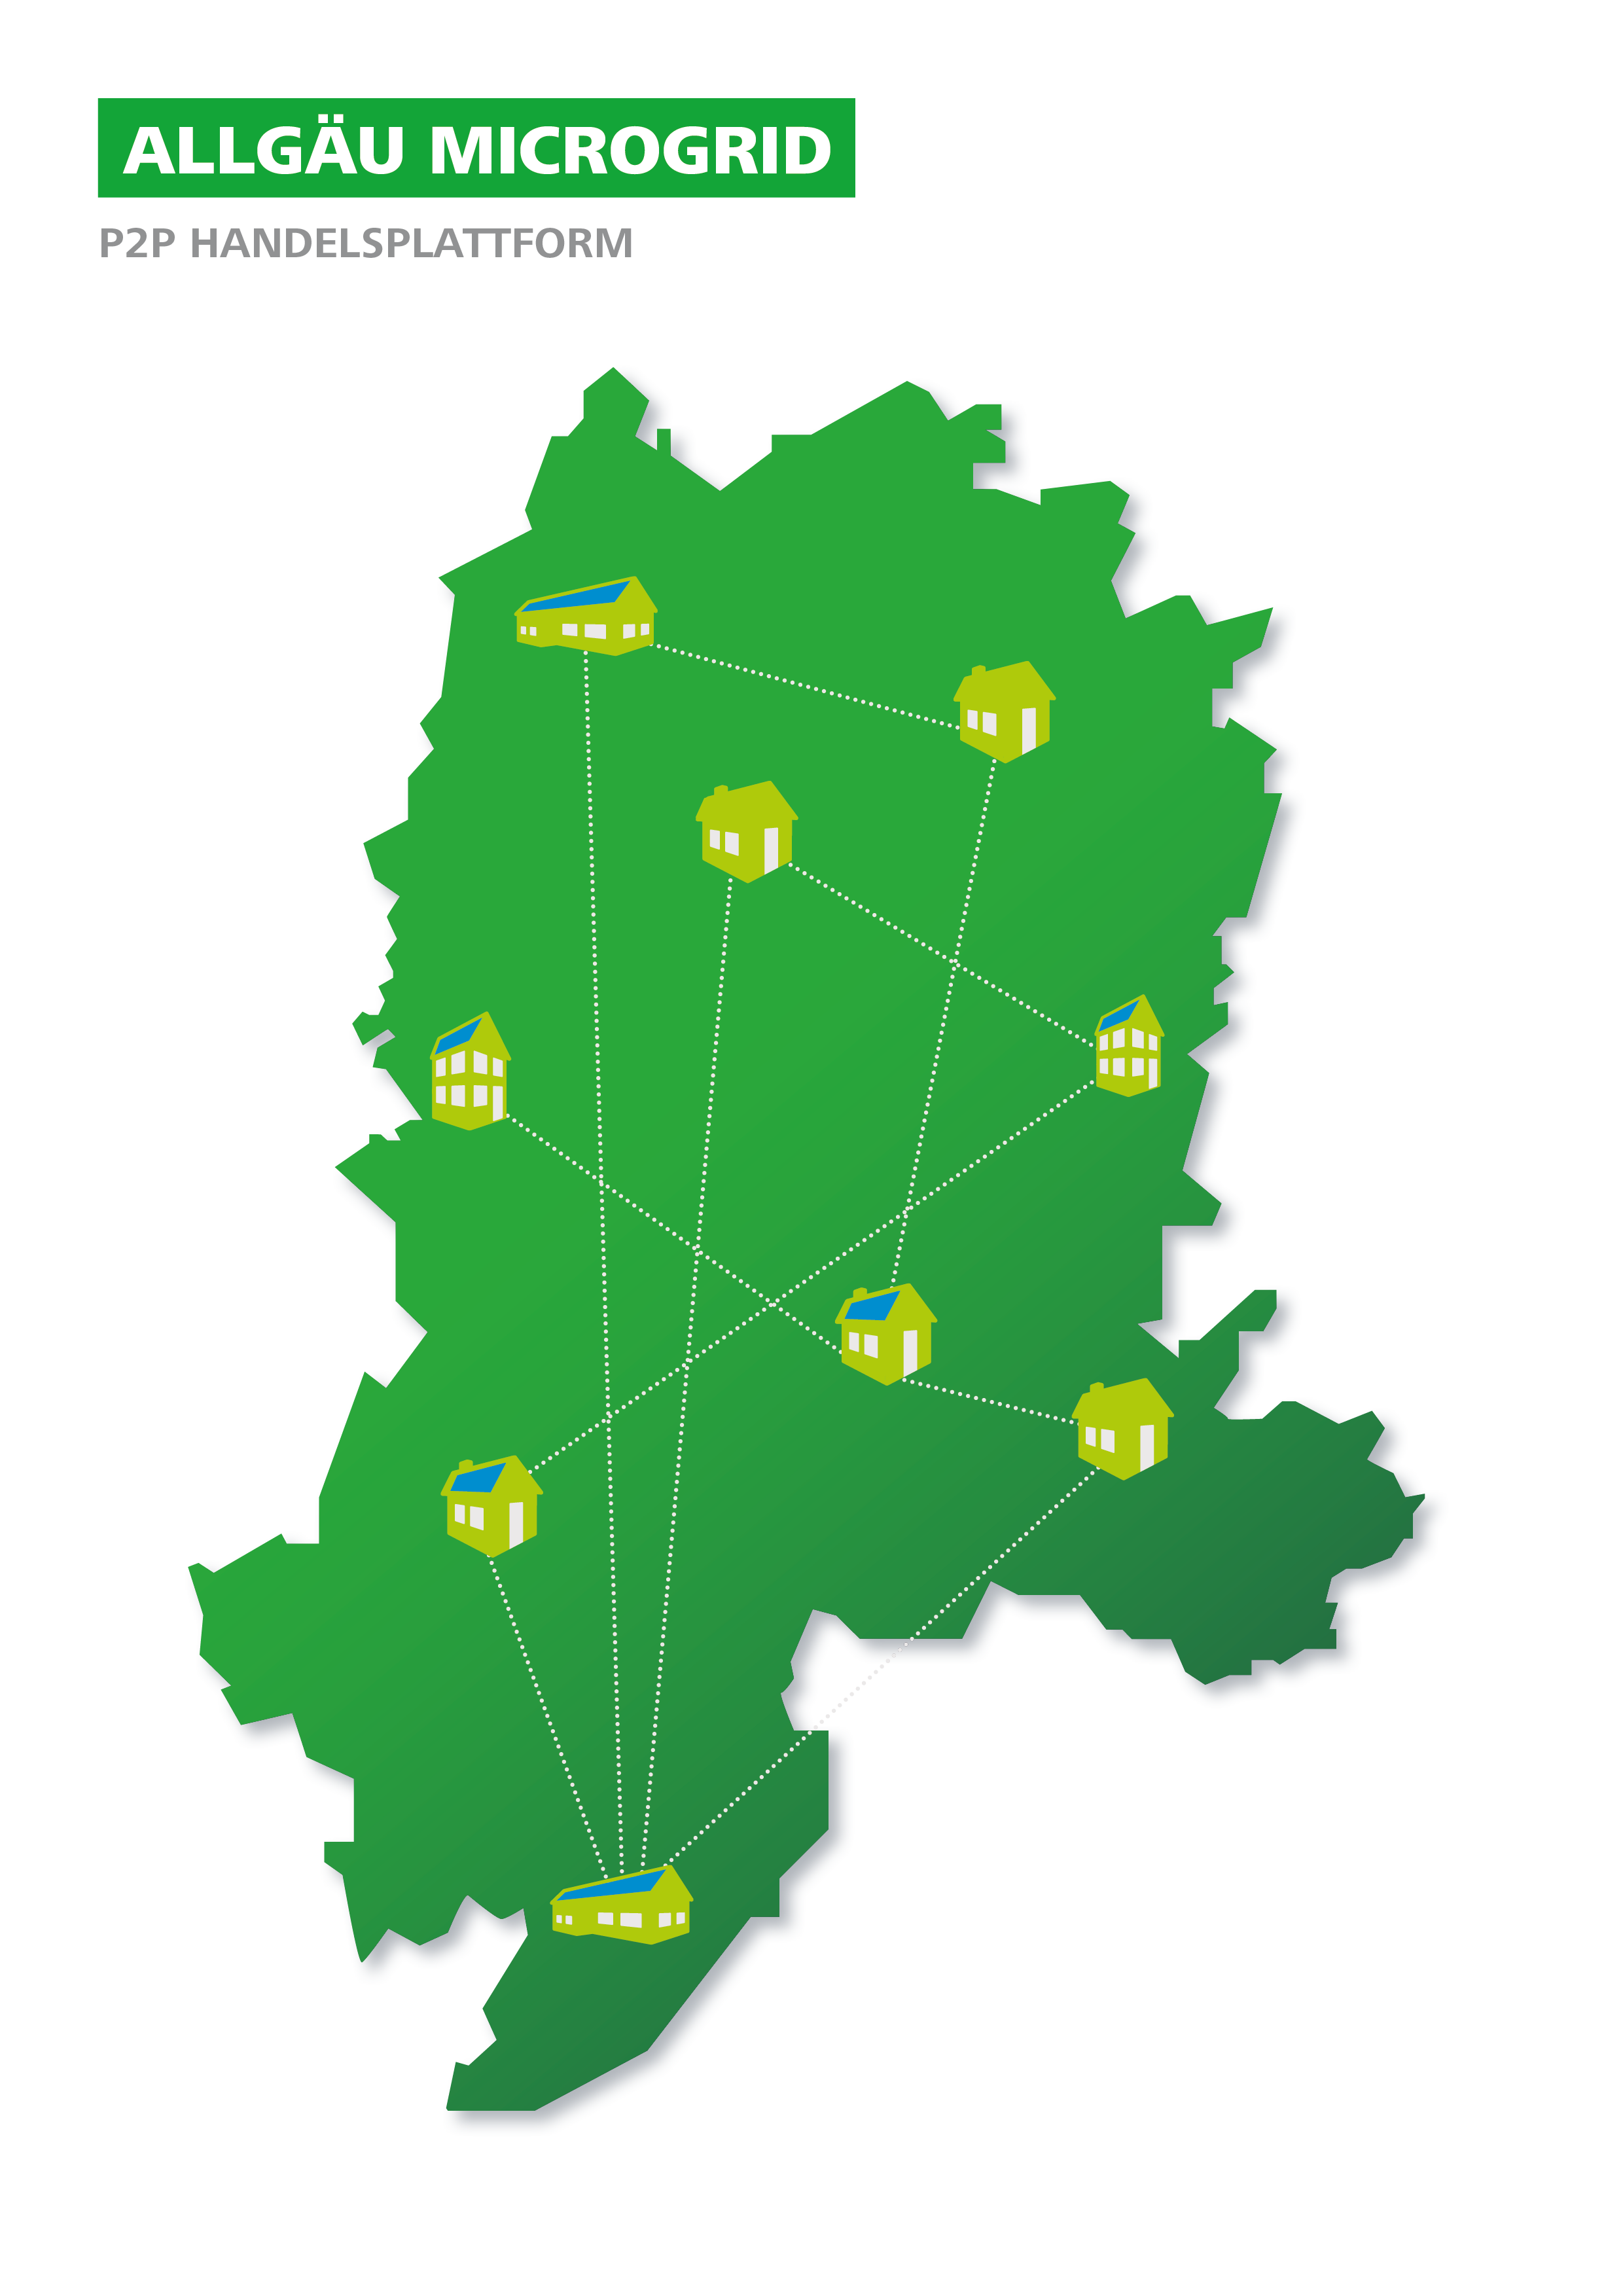
\includegraphics[width=.4\textwidth]{Bilder/Microgrid.png}
  \caption[Microgrid]{Microgrid \cite{AÜW}}
  \label{fig:Microgrid}
\end{wrapfigure}

Eines der dort durchgeführten Projekte ist das sogenannte \emph{Allgäu Microgrid} aus Abbildung \ref{fig:Microgrid}. Ziel dieses Grids (engl., hier gemeint: Stromnetz) ist es, eine Plattform für den Peer to Peer Stromhandel zu entwickeln. Dafür wurde die Partnerschaft mit LO3-Energy aus New York gesucht, welche mit dem Brooklyn Microgrid bereits eine ähnliche Plattform aufgebaut haben \cite[vgl.][]{BrooklynGrid2019}. Welche Blockchain-Lösung dafür eingesetzt wird, wird nicht erwähnt. Im Allgäu soll das Grid vor allem auf die Zeit nach dem Erneuerbare Energien Gesetz abzielen, d.h. wenn die staatliche Förderungen für Votovoltaikanlagen so weit zurück geht, dass eine Rentabilität nicht mehr gegeben ist. Deshalb wird mithilfe von fünf Pilotkunden eine Plattform in der Ortschaft Wiggensbach im Allgäu aufgebaut, welche zum Stromhandel dient. Daran sind sowohl Anlagenbesitzer (Prosumer, Producer + Consumer) als auch reine Konsumenten (Consumer) beteiligt. Fällt bei den Prosumern überschüssige Energie an, kann diese über das Netzwerk an Andere verkauft werden. Bisher wird der Strom wieder beim Energieversorger eingespeist, wofür das Erneuerbare-Energien-Gesetz die Grundlage bildet. Aufgrund von fallender Bezuschussung wird der Rückerverkauf von Strom aber immer unrentabler. Bei dem Microgrid hingegen können beide Seiten einen Schwellwert festlegen, bei dem verkauft bzw. angekauft werden soll. Kommt es zu einem Matching von Angebot und Nachfrage mithilfe eines Smart Contracts, wird die Umverteilung in die Wege geleitet. Um das bewerkstelligen zu können, werden einige technische Grundvoraussetzungen gestellt. Dazu zählt unter anderem auch ein DSL-Anschluss mit einer Übertragungsleistung von 16 000 MBit/s. Des Weiteren benötigen sowohl Prosumer als auch Consumer ein Messsystem, welches die Daten über den Verbrauch des Stroms bzw. dessen Erzeugung an die Plattform übermittelt. Dieses wird vom AÜW kostenlos zur Verfügung gestellt. Um den bereits genannten Ein- bzw. Verkaufswert angeben zu können, wird eine Smartphone-/Tablet-App benötigt. Daher sollen vor allem technik-affine Menschen angesprochen werden. \cite[vgl.][]{AÜW, Klaus2018}

Dieses bereits abgeschlossene Projekt dient als Vorlauf für das seit 2018 drei Jahre andauernde Forschungsprojekt \emph{Pebbles}. Daran sind neben dem AÜW auch die Hochschule Kempten, das Fraunhofer Institut, Siemens und Allgäu Netz beteiligt. Hier sollen die Möglichkeiten eines Peer to Peer Stromhandels weiter erforscht werden, z.B. indem auch Firmen an die Plattform und somit auch an die Blockchain-Lösung angeschlossen werden. Auch die bisher eingesetzen Smart Contracts sollen ausgeweitet werden, um ein breiteres Funktionssprektrum anbieten zu können. So soll neben einer lokalen Umverteilung des Stroms auch an einer Strombörse Handel betrieben werden. Dazu kommen weitere Applikationen, z.B. für Data Mining, welche die Daten der Plattform weiterverarbeiten können. \\
Hürden, wie die in anderen Bereichen bereits angesprochene DSGVO soll auch zu einer ganzheitlichen Klärung der Thematik beitragen. Nach den theoretischen Vorarbeiten sollen die Konzepte auch schlussendlich simuliert werden, um die Praxistauglichkeit überprüfen zu können. \cite[vgl.][]{Ziegler2018}

Die angestrebten Plattformen des AÜW sind nur ein Beispiel für den Fortschritt in der Digitalisierung und dem damit involvierten Einsatz von Technologien wie Smart Contracts. Auch in anderen Städten in Deutschland wird bereits an Ähnlichem geforscht; in anderen Ländern wie beispielsweise Norwegen ist der smarte Umgang mit Energie und Elektromobilität bereits Alltag. \\
Leider war es auch in diesem Beispiel nicht möglich, Einblicke in die Smart Contracts zu erhalten, was sich aber unter Anbetracht der gewünschten Sicherheitsaspekte bei Energieplattformen durchaus verständlich ist. Zudem stellen solche innovativen Ansätze Vorteile gegenüber der Konkurrenz da, weshalb oftmals keine Öffnung des Programmcodes stattfindet. \\
Inwiefern sich Vorteile durch den Einsatz von Blockchains und Smart Contracts ergeben, wird zudem durch Pebbles von verschiedenen Seiten beleuchtet. Daher wird sich zeigen, ob solche neuen Plattformen die gewünschten Effekte und Ansprüche erfüllen können.